\documentclass[10pt,a4paper]{article}
\usepackage[utf8]{inputenc}
\usepackage[english]{babel}
\usepackage{graphicx}
\usepackage{mathtools}
\usepackage{todonotes}

\author{Jonathan Dan}

\newcommand{\bookref}[2]{\indent\indent\indent\indent $\vert\vert$ Book reference: ``#1'' (pp. #2) \newline}

\begin{document}

\section{Chapter 8 - Sensor interface and bus system}

\subsection{What is cross-sensitivity? Give two compensation techniques cross-sensitivity.}

\bookref{8.3.2 Cross-sensitivities}{403-406}

When a sensor is sensitive to an undesirable parameter we say this sensor as a cross-sensitivity to that parameter.\newline

Solutions:
\begin{itemize}
	\item Design a sensor in such a way that some parts of the sensor have a temperature (or any other parameter) coefficient which is opposite to other parts. Eg. Wheatstone bridge where two resistors have a positive temperature coefficient and two have a negative temperature coefficient or amplifier with a temperature coefficient opposite to sensor temperature coefficient.
	\item Add a sensor measuring the undesirable parameter. Correct the output of the main sensor using the measure of the undesired parameter. Eg. Pressure sensors are often temperature dependent, add a temperature sensor and compensate the measured the pressure.
\end{itemize}
Other examples: Switching current and voltage contacts in a Hall plate (same as electronic instrumentation)

\subsection{Give a block-diagram of a sensor bus system, with single and multi sensor modules.}

\bookref{8.6.3 Bus systems}{424-426}

\begin{figure}[h!]
    \centering
    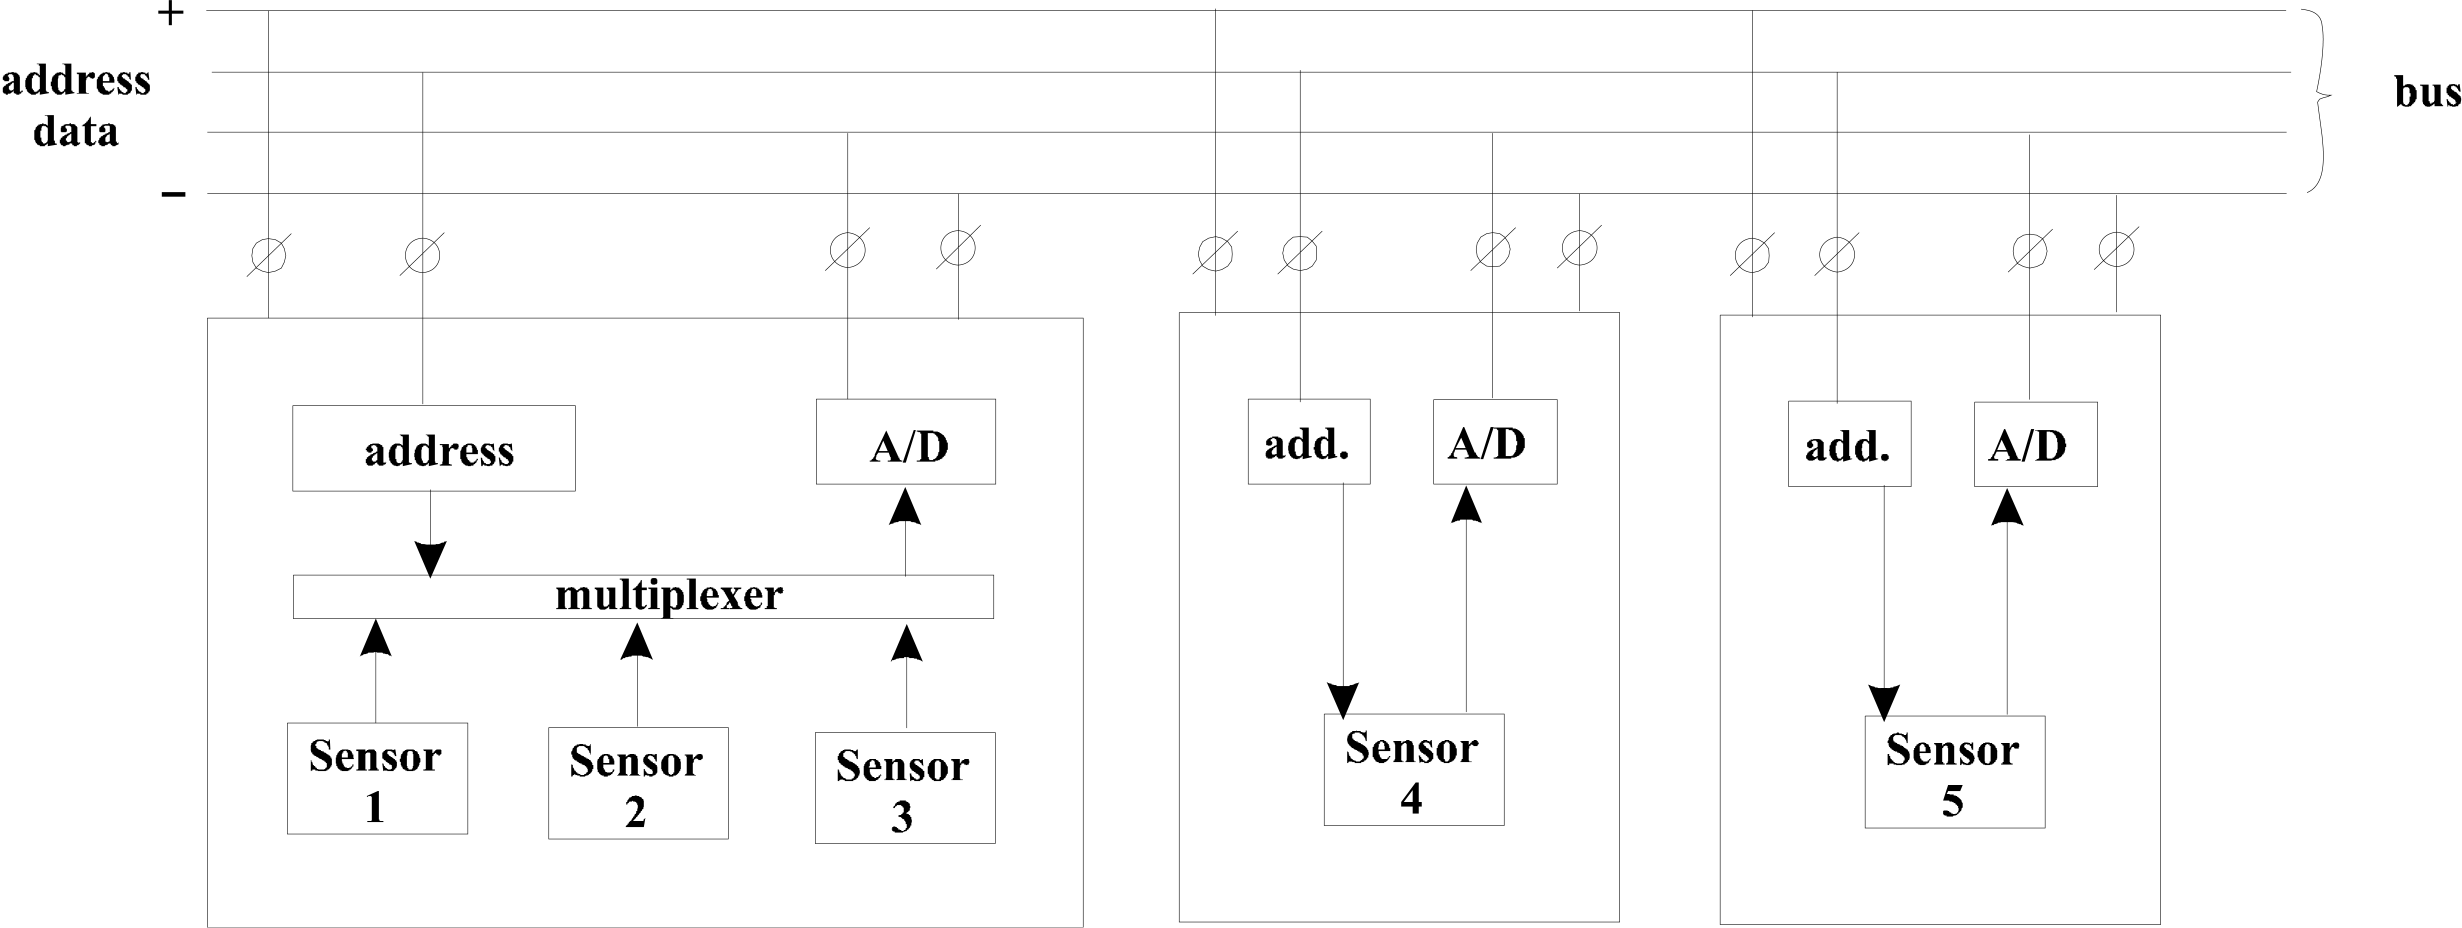
\includegraphics[width=\textwidth]{bus.png}
    \caption{Digital sensor bus interface structure}
\end{figure}

\subsection{Draw a Wheatstone-bridge for pressure measurement with all four resistors used as a sensor give the expression of for the output signal. Each resistor has a temperature coefficient of resistance and also for mechanical stress. Give the expression for the output signal for an elevated temperature. Is there a difference if the bridge is powered by constant voltage or constant current? Why?}

\begin{figure}[h!]
    \centering
    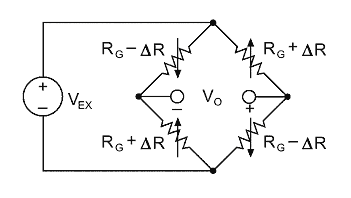
\includegraphics{bridge.png}
    \caption{Wheatstone bridge - 4 varying resistors}
\end{figure}

\begin{equation} \label{eq:wheatstone}
	V_{O} = V_{EX}.\frac{\Delta R}{R}
\end{equation}

If the temperature coefficient is the same for all sensors then they will be no change to the output. If two are positive and two are negative the change in output voltage is equal to (\ref{eq:wheatstone}).

No they would be no difference if the bridge was powered by constant current or voltage. This can be seen by doing the same calculation with a current source.

\todo{3 questions to integrate}
\todo{Integrate question: ``Why is a Wheatstone bridge used fro pressure measurement? Draw a bridge with one, two and four sensing resistors and give formula for the output signal. Each resistor is sensitive to temperature sensitive. How can we make this cross sensitivity as small as possible?''}
\todo{Integrate question: ``Compare the output and temperature coefficient of a Wheatstone bridge based piezoresistive pressure sensor, with; a) 1 resistor as sensor, b) 2 resistors as sensor and c) all 4 resistors as sensor.''}
\todo{Integrate question: ``How can temperature sensitivity be reduced in a pressure sensor based on piezoresistors?''}

\subsection{How does the ``sensitivity variation method'' work to reduce offset? In which circumstances does this not bring the offset to zero?}

\bookref{8.3.1.1 Sensitivity-variation offset-reduction method}{401-403}

\[ V_{out} = S_{entivity}M_{easure} + O_{ffset} \]

By applying a modification to the sensor (thus to the sensitivity). Two output values can me found for the same measure. This allows us to calculate the offset. If we know the offset we can simply subtract it to the value reported by the sensor.

\[
\begin{cases} V_1 = S_1M + O  \\ V_2 = S_2M+O \end{cases} \iff
\begin{cases} M = \frac{V_2-V_1}{S_2-S_1}  \\ O = \frac{S_2 V_1 - S_1 V_2}{S_2 - S_1} \end{cases} 
\]

These modifications could be a change in temperature or in the surrounding magnetic field, etc.

However this technique only works if the modification we apply to the sensor does not affect the offset.

\subsection{What is the basic principle of a flip-flop sensor? What are the advantages and disadvantages of this technique?}

\bookref{8.4.2.3 Stochastic analogue-to-digital converters}{415-417}

An equally distributed number of `1' and `0' can be generated at the output of a flip-flop circuit by switching on and off the supply voltage the circuit. This is due to the noise in the  flip-flop circuit components. However, if an asymmetry is introduced in the circuit this distribution will no longer be equally distributed. By counting the number of `1' and `0' it is possible to measure the asymmetry in the circuit. Figure \ref{fig:flip-flop} shows two sensors based on the flip-flop circuit.

\begin{figure}[h!]
    \centering
    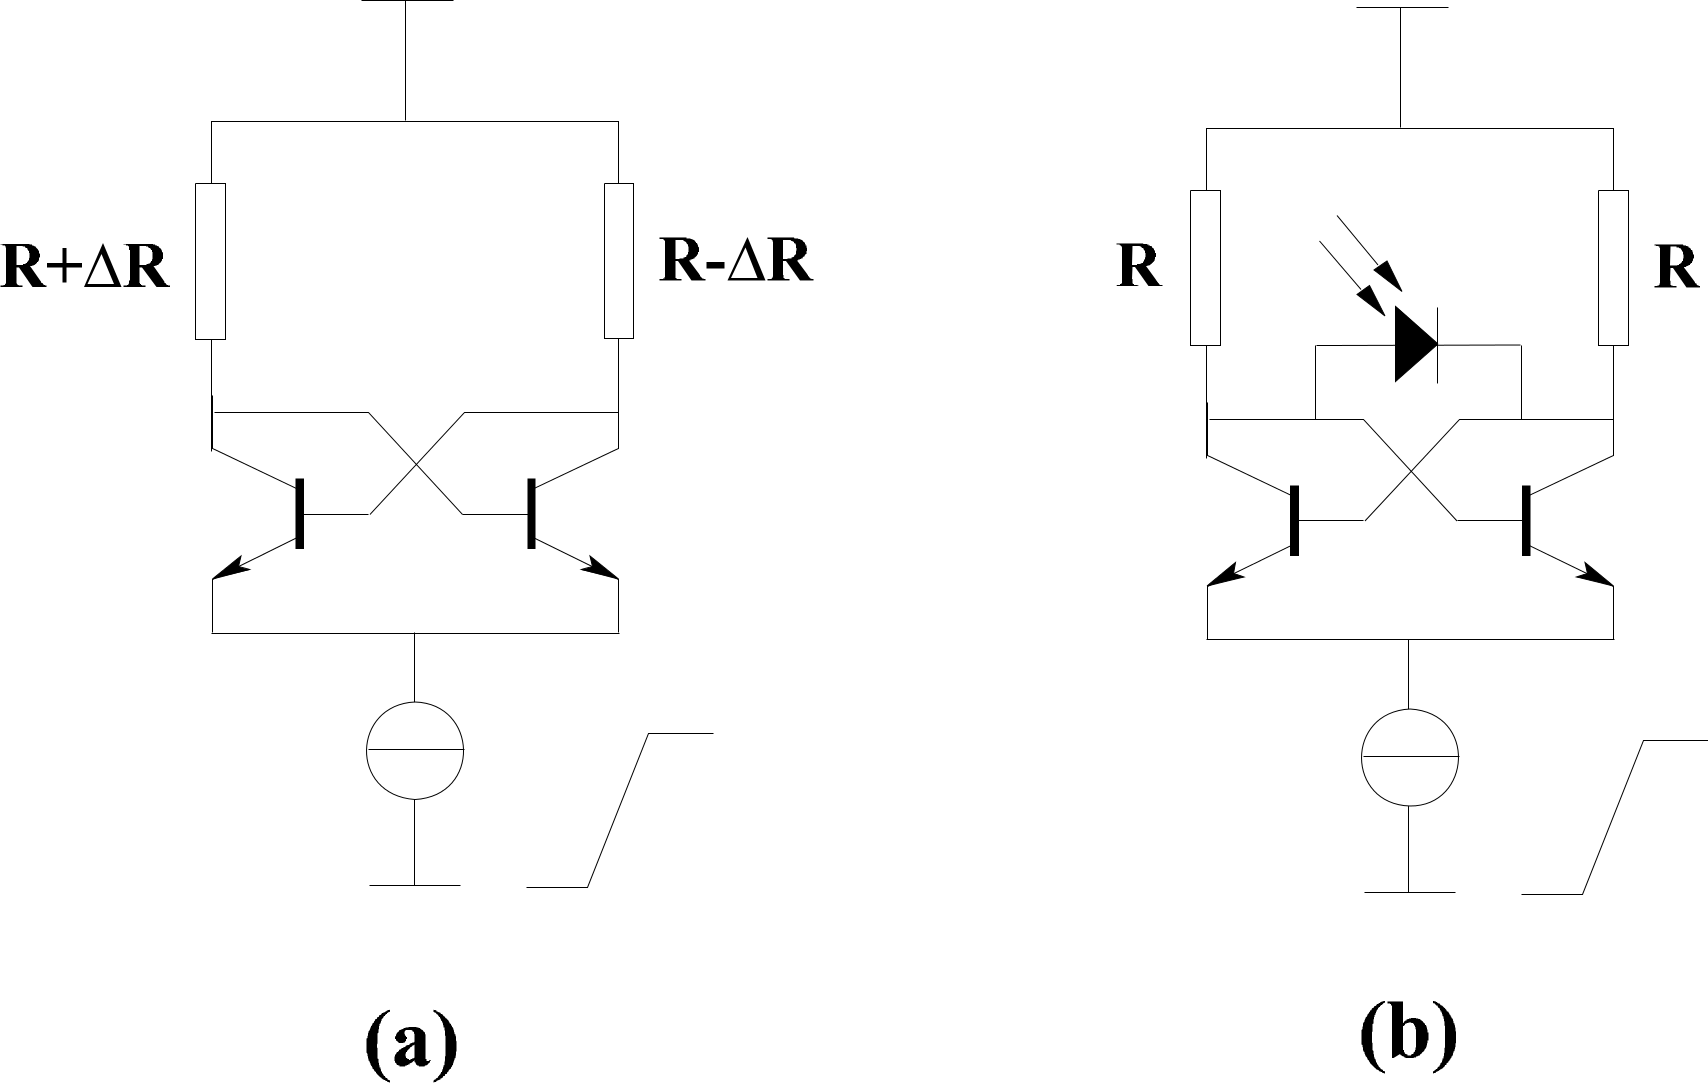
\includegraphics{flip-flop.png}
    \caption{(a) Pressure sensitive flip-flop, (b) light-sensitive flip-flop}
    \label{fig:flip-flop}
\end{figure}

A flip-flop sensor as the advantage of being highly accurate and immune to noise (binary output). The output of the flip-flop sensor is easy to interpret (count pulses). Flip-flop circuits are small so they can easily be arranged in arrays.

A disadvantage of the flip-flop circuit is that the input signal must be stationary for an amount of time that is long enough to produce enough supply voltage pulses to generate an equally distributed number of `1' and `0' at rest. 

\subsection{How can a ring-oscillator be used as a sensor? Give two examples.}

\textit{No reference in book}\\

A ring oscillator is a device composed of an odd number of NOT gates. The output is fed back to the input to create an oscillating circuit (period is twice -- full cycle -- the delay of each gate gate).

\begin{figure}[h!]
    \centering
    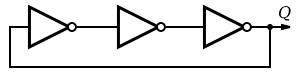
\includegraphics{ring.png}
    \caption{3-inverter ring oscillator whose output frequency is 1/(6xinverter delay}
\end{figure}

\begin{description}
	\item[Temperature] If the NOT gates are built using CMOS technology a linear dependency is introduced between the oscillation frequency and the bias current. If the bias current is temperature dependant, then oscillation frequency and temperature are dependant. [source: S. Suman and B.P. Singh, ``Design of Temperature Sensor Using Ring Oscillator'', \textit{International Journal of Scientific \& Engineering Research}, Vol.3:5, 2012]
	\item[Pressure] By building a CMOS ring oscillator which includes a MEMS pressure sensing capacitance it is possible to build a pressure sensitive ring oscillator. This is illustrated in figure \ref{fig:ring-cap}. [source: Ching-Liang Dai, Po-Wei Lu , Chienliu Chang and Cheng-Yang Liu, ``Capacitive Micro Pressure Sensor Integrated with a Ring Oscillator Circuit on Chip'', \textit{Sensors}, pp. 10158-10170, Sept 2009]
\end{description}

\begin{figure}[h!]
	\centering
	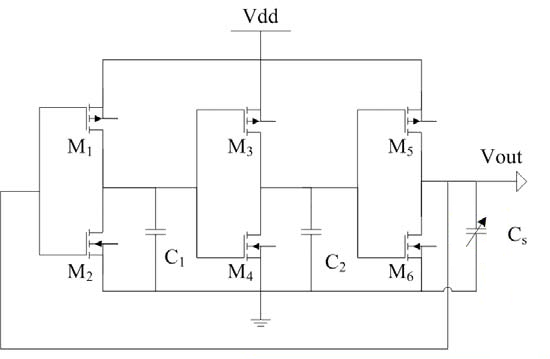
\includegraphics[width=\textwidth]{ring-cap.png}
	\caption{Pressure sensing ring oscillator}
	\label{fig:ring-cap}
\end{figure}

\subsection{A sensor signal can be converted into a frequency. Give three methods to generate a frequency output from a
sensor signal.}

\begin{enumerate}

	\item A voltage controlled oscillator. Using a switch to charge and discharge a variable capacitor. This gives a triangular type wave, which can be converted into a square wave using a comparator.
	\item A ring oscillator - a ring oscillator contains an odd number of inverters with a feedback loop. The oscillator will give a frequency output with a frequency determined by the number of inverters and the switching time of each inverter. If we can make the switching time a function of the measurand, we have a frequency output sensor. One example is the pressure sensor using CMOS. If the inverters are stressed, the switching time is changed due to the piezoresistive effect in the channel.
	\item A SAW device. Surface acoustic waves are sent over the surface of the device using a piezoelectric material. The time wave takes to travel from the sender to the receiver can be made to be a function of the measurand. For example, for measuring liquid density, where a more dense liquid will slow down the wave's progress. If we feed this output back to the input, we can generate a frequency, which is a function of the speed of the wave over the surface
\end{enumerate}

\end{document}